\documentclass[11pt, a4paper, oneside]{article}

\usepackage{pifont}
\newcommand{\cmark}{\ding{51}}
\usepackage{tikz}
\usetikzlibrary{arrows, automata}

\begin{document}

\title{Homework 3}
\author{Aaron Rosen}
\date{Tuesday, March 6}
\maketitle

\section*{Problem 1 (Kozen HW3 \#1)}
\subsection*{(a)}
$L = \{ a^n b^m | n = 2m\}$
Let $k$ be given. Let $x = a^{2k}$, $y = b^k$ and $z = E$. 
	Note that $xyz = a^{2k} b^k \in L$. Let $y = uvw$, where $|u| = i$, $|v| = j$,
	$|w| = l$, and $v \neq E$. Then $k = i + j + l$ and $j > 0$. \\

$xuv^rwz = a^{2(i+j+l)}uv^rw$\\
\\
When $r = 1$ then $|uvw| = |y| = k$ but choose any other $r > 1$ and $|y| > k$ 
	and more importantly $|y| \neq \frac{1}{2}|x|$ which means the string is no
	longer in the language.
\subsection*{(b)}
$L = \{x \in \{a, b, c\}^* | x$ is a palendrome; i.e., $x = $rev$(x)\}$\\
Suppose for the sake of contradiction, $L$ is regular. Then \\

$L \cap a^* b^* a^* = \{a^n b^m a^n\}$\\
\\
Which we know is not regular, so $L$ is not regular.
\subsection*{(c)}
$L = \{x \in \{a, b, c\}^* | $ the length of $x$ is a square $\}$\\
Let $k$ be given and $k$ is a square. Let $x \in L$ so $|x| = k$. Let's 
	say $x=rt$, where $r = \{a, b, c\}$ and $|t| = k - 1$,\\

$x = r^2 t \notin L$\\
\\
because if $k$ is a square then $|x| = k - 1 + 2 = k + 1$ is not a square.
\subsection*{(d)}
$P = \{ x \in \{$")"$,$"("$\} | \forall$ $ "("$ there 
	is exactly one $")"$ following $\}$\\
Let $a = $"(" and $b = $ ")" then $L(a^* b^*) \cap P = L(a^n b^n)$ which we know
	is not regular so $P$ must not be regular.

\section*{Problem 2 (Kozen HW3 \#2)}
\subsection*{(a)}
$(01)^* || (10)^* = ((01) + (10) + (11)(00) + (00)(11))^*$

\subsection*{(b)}
Let $M_A$ and $M_B$ be machines: \\
\\
$M_A = (Q_A, \Sigma, \delta _A, S_A, F_A)$\\
$M_B = (Q_B, \Sigma, \delta _B, S_B, F_B)$\\
\\
where $M_A$ is the macing accepting the language $A$ and $M_B$ is the machine
accepting the language $B$. \\
We can define the macine that accepts the language $A||B$ as: \\

$M_{AB} = (Q_A \times Q_B, \Sigma, \delta _{AB}, S_A \times S_B, F_A \times F_B)$ 
where $p \in Q_A$ and $q \in Q_B$. \\

$\delta _{AB} ([p,q],a) = \{[\delta _A (p,a),q],[p, \delta _B (q,a)]\}$\\

\textbf{\underline{Lemma 1}}
Given an arbitrary state $[p,q]$, applying the transition function with 
some $a \in \Sigma$ either moves state $p$ via $M_A$'s transition function
to some $p' \in Q_A$, leaving $q$ in place, or moves state $q$ via $M_B$'s
transition function to some state $q' \in Q_B$, leaving $p$ in place.\\
\\
Starting at some state $[s_a, s_b] \in S_A \times S_B$ with some $x \in \Sigma^*$.
According to lemma 1, for each letter of $x$, $\delta _{AB}$ will return some 
state in $Q_A \times Q_B$. If, after the last letter in $x$, $q' \in F_B$ and 
$p' \in F_A$ then $x \in L(A||B)$. Therefore $A||B$ must be regular.


\section*{Problem 3 (Kozen HW3 \#3)}
\subsection*{(a)}
In the first machine only 7 and 8 are inaccessible, in the second all states 
are accessible.

\subsection*{(b)}
\begin{tabular}{c c}
\begin{tabular}{*{10}{c}}
\hline
1 \\
\cmark & 2 \\
\cmark & \cmark & 3 \\
\cmark & \cmark & & 4 \\
\cmark & & \cmark & \cmark & 5 \\
 		   & \cmark & \cmark & \cmark & \cmark & 6 \\
\cmark & \cmark & \cmark & \cmark & \cmark & \cmark & 7 \\
\cmark & & \cmark & \cmark & & \cmark & \cmark & 8 \\
\hline
\end{tabular}
&
\begin{tabular}{*{10}{c}}
\hline
1 \\
 & 2 \\
\cmark & \cmark & 3 \\
\cmark & \cmark & & 4 \\
\cmark & \cmark & \cmark & \cmark & 5 \\
\cmark & \cmark & \cmark & \cmark & & 6 \\
\cmark & \cmark & \cmark & \cmark & & & 7 \\
\cmark & \cmark & & & \cmark & \cmark & \cmark & 8 \\
\hline
\end{tabular}
\\
$[3] = \{3,4\}$, $[2] = \{2,5,8\}$, $[1] = \{1,6\}$
&
$[1] = \{1,2\}$, $[3] = \{3,4,8\}$, $[5] = \{5,6,7\}$
\end{tabular}
\subsection*{(c)}
\begin{tabular}{c c}
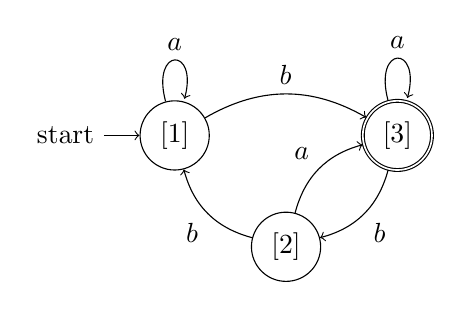
\begin{tikzpicture}[auto, node distance=2cm]
	\node[initial, state] 	(one)                        {$[1]$};
	\node[state]            (two)   [below right of=one] {$[2]$};
	\node[state, accepting] (three)	[above right of=two] {$[3]$};

	\path[->] (one) edge[loop above] node {$a$} (one);
	\path[->] (one) edge[bend left] node {$b$} (three);
	\path[->] (two) edge[bend left] node {$a$} (three);
	\path[->] (two) edge[bend left] node {$b$} (one);
	\path[->] (three) edge[loop above] node {$a$} (three);
	\path[->] (three) edge[bend left] node {$b$} (two);
\end{tikzpicture}
&
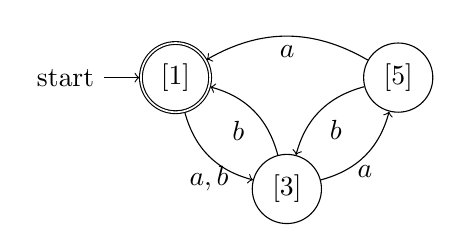
\begin{tikzpicture}[auto, node distance=2cm]
	\node [initial, state, accepting] (one) 													{$[1]$};
	\node [state]											(three)  [below right of=one]  	{$[3]$};
	\node [state]											(five)   [above right of=three] {$[5]$};

	\path[->] (one) edge[bend right] node[below] {$a,b$} (three);
	\path[->] (three) edge[bend right] node[below] {$a$} (five);
	\path[->] (three) edge[bend right] node {$b$} (one);
	\path[->] (five) edge[bend right] node {$a$} (one);
	\path[->] (five) edge[bend right] node {$b$} (three);
\end{tikzpicture}
\end{tabular}
\end{document}


